\begin{figure}[t]
 \centering
 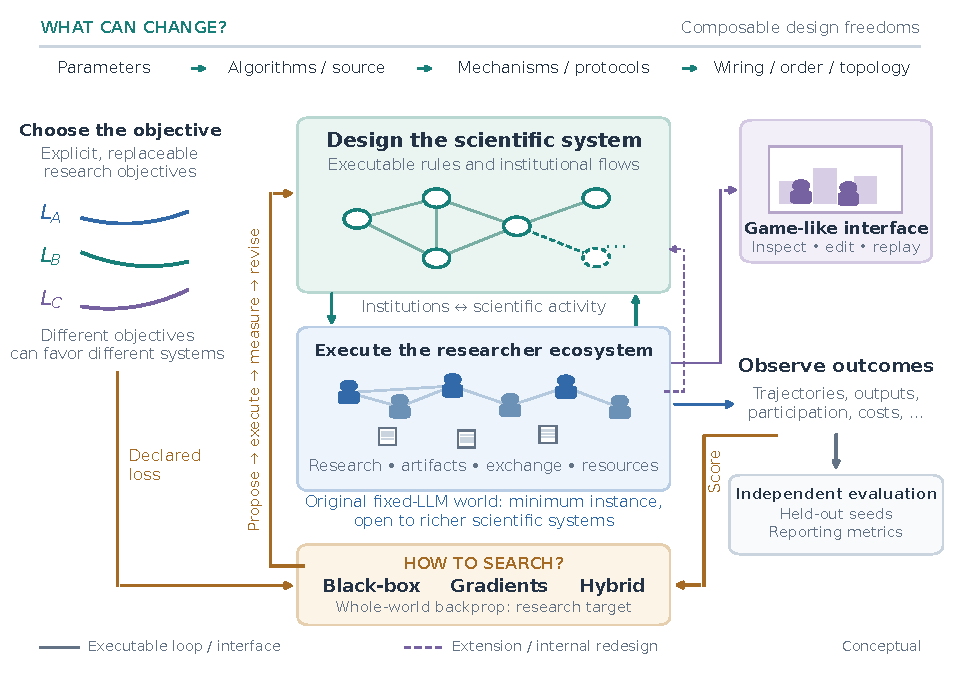
\includegraphics[width=\linewidth]{figures/program-concept/science-system-design-program.pdf}
 \caption{\textbf{Scientific systems as objects of design: the research program.}
 An explicit objective conditions the search for a scientific system.
 Design freedom extends from parameters to executable algorithms, new
 mechanisms and protocols, wiring and execution order. These freedoms compose;
 search methods form a separate axis. Differentiable representations target
 the same research world rather than replacing it with a simpler toy.
 The original fixed-LLM researcher world is a minimum
 contained instance, not a simpler substitute for the intended ecosystem.
 Outcomes feed the optimizer, while independent evaluation metrics remain
 separate from the optimized loss. The game-like interface supports inspection,
 editing and replay. Solid connections denote executable paths, not successful
 scientific invention. Dashed connections indicate research targets, including
 internal redesign. Useful autonomous institutional invention and whole-world
 backpropagation are goals, not established results. Curves and layouts are
 conceptual, not empirical data.}
 \label{fig:research-program}
\end{figure}
